% !TeX program = pdflatex
%==============================================================================
%  Aula 09 --- Máquinas de Vetores de Suporte (SVM) --- SLIDES
%
%  Origem: deck em Beamer do Prof. Hugo Tremonte de Carvalho (UFRJ), recebido
%  em 17/08/2026 num zip com o main.tex do curso inteiro dele (137 frames) e 50
%  figuras. Deste arquivo saíram só os 30 frames de SVM -- os outros 107, que no
%  main.tex estavam dentro de \begin{comment}, ficaram de fora, e com eles 40
%  figuras que nenhum frame daqui usa.
%
%  Três mudanças em relação ao recebido, e o motivo de cada uma:
%
%    1. autoria e instituição: Gabriel Sanfins / UFF no lugar de Hugo Carvalho /
%       UFRJ. O rodapé das 31 páginas sai de \author[...] e \title[...], então
%       são as duas chaves curtas que importam. O título curto também perdeu o
%       "Apredizagem" (faltava o n) e passou a "Aprendizado de Máquina", que é
%       o nome do curso no resto do repositório;
%    2. o \usepackage[portuguese]{babel} saiu, e "Figura" é definido à mão. É a
%       mesma decisão do recursos/latex/estilo-notas.sty, e por um motivo
%       prático: sem o texlive-lang-portuguese o babel falha em silêncio e as
%       legendas voltam para "Figure". Sem babel, compila igual em qualquer
%       máquina -- ao preço de não haver hifenização portuguesa;
%    3. inputenc utf8x -> utf8 (o utf8x depende do ucs, que está obsoleto) e as
%       figuras num subdiretório, via \graphicspath.
%
%  As citações [ITSL] viraram [ISLP] -- é o mesmo livro, e é a sigla que os
%  outros seis decks do curso já usam desde 10/08/2026.
%
%  Compile de dentro desta pasta:  pdflatex "10 SVM - slide.tex"
%==============================================================================
\documentclass[handout]{beamer}
% \documentclass{beamer}

\mode<presentation>
{
  \usetheme{Madrid}
  \usecolortheme{beaver}
  \usefonttheme{serif}
  \setbeamertemplate{navigation symbols}{}
  \setbeamertemplate{caption}[numbered]
} 

\usepackage{pgfpages}
\setbeameroption{hide notes} % Only slides
% \setbeameroption{show oly notes} % Only notes
% \setbeameroption{show notes on second screen=right} % Both
\setbeamertemplate{note page}{\pagecolor{yellow!5}\insertnote}%\usepackage{palatino}

% babel fora de propósito: ver o cabeçalho deste arquivo
\usepackage[utf8]{inputenc}
\renewcommand{\figurename}{Figura}
\renewcommand{\tablename}{Tabela}
\usepackage{xcolor}
\usepackage{listings}
\usepackage{booktabs}
\usepackage{comment}
\usepackage{graphicx}
\graphicspath{{slide-figuras/}}
\usepackage{bm}
\usepackage{ulem}
\lstset
{
    language=[LaTeX]TeX,
    breaklines=true,
    basicstyle=\tt\small,
    %commentstyle=\color{green}
    keywordstyle=\color{blue},
    %stringstyle=\color{black}
    identifierstyle=\color{magenta},
}

 \setbeamertemplate{footline}
        {
      \leavevmode%
      \hbox{%
      \begin{beamercolorbox}[wd=.3\paperwidth,ht=2.25ex,dp=1ex,center]{author in head/foot}%
        \usebeamerfont{author in head/foot}\insertshortauthor
      \end{beamercolorbox}%
      \begin{beamercolorbox}[wd=.4\paperwidth,ht=2.25ex,dp=1ex,center]{title in head/foot}%
        \usebeamerfont{title in head/foot}\insertshorttitle
      \end{beamercolorbox}%
      \begin{beamercolorbox}[wd=.3\paperwidth,ht=2.25ex,dp=1ex,right]{date in head/foot}%
        \usebeamerfont{date in head/foot}\insertshortdate{}\hspace*{2em}
        \insertframenumber{} %/ \inserttotalframenumber
        \hspace*{2ex} 
      \end{beamercolorbox}}%
      \vskip0pt%
    }

%---------- MY DEFINITIONS ----------%
\newcommand{\V}[1]{{\bf #1}} % Bold math symbol
\newcommand{\Vg}[1]{\bm{#1}} % Bold math symbol (for greek letters)
\newcommand{\sumint}[1]{\sum\limits_{#1 = -\infty}^{+\infty}} % Sum from -infty to +infty. The argument of the command is the summation variable

% To write bold math symbol for greek letter in title of sections, the command "\vect" must be used!
\DeclareRobustCommand{\vect}[1]{\bm{#1}}
%\pdfstringdefDisableCommands{%
	\renewcommand{\vect}[1]{#1}%
%}

\def \j {\cap} % Intersection
\def \u {\cup} % Union

%-- ENVIRONMENT FOR QUESTION --%
\newcounter{questctr}
\newenvironment{question}{%      define a custom environment
	\noindent%         create a vertical offset to previous material
	\refstepcounter{questctr}% increment the environment's counter
	\textbf{Questão \thequestctr:}% or \textbf, \textit, ...
}{\par\bigskip}  %          create a vertical offset to following material
%\numberwithin{questctr}{section}
%-- ENVIRONMENT FOR QUESTION --%

% Double and triple integrals with integration limits
\newcommand{\intd}[4]{\int_{#1}^{#2}\int_{#3}^{#4}}
\newcommand{\intt}[6]{\int_{#1}^{#2}\int_{#3}^{#4}\int_{#5}^{#6}}

% Letters to denote the real number set, integers, expectation operation, etc.
\def \CC {\mathbb{C}}
\def \EE {\mathbb{E}}
\def \GG {\mathbb{G}}
\def \II {\mathbb{I}}
\def \NN {\mathbb{N}}
\def \PP {\mathbb{P}}
\def \QQ {\mathbb{Q}}
\def \RR {\mathbb{R}}
\def \VV {\mathbb{V}}
\def \ZZ {\mathbb{Z}}

% Manuscript letters
\def \Bcal {\mathcal{B}}
\def \Ccal {\mathcal{C}}
\def \Fcal {\mathcal{F}}
\def \Gcal {\mathcal{G}}
\def \Hcal {\mathcal{H}}
\def \Ncal {\mathcal{N}}
\def \Lcal {\mathcal{L}}
\def \Tcal {\mathcal{T}}
\def \Vcal {\mathcal{V}}
\def \Wcal {\mathcal{W}}
\def \GPcal {\mathcal{G}\mathcal{P}}

\def \diag {\text{diag}}

% convergence in probability
\def \convprob {\overset{p}{\to}}

% convergence almost sure (in portuguese)
\def \convqc {\overset{qc}{\to}}

% convergence almost sure (in english)
\def \convas {\overset{as}{\to}}

% convergence in distribution
\def \convdist {\overset{d}{\to}}

% convergence in r mean, with different values of r
\newcommand{\convr}[1]{\overset{#1}{\to}}

% theta hat (for estimators)
\def \thetahat {\hat{\theta}}

% erro medio quadratico (in Portuguese)
\def \eqm {\mathrm{EQM}}

% quadratic mean error (in English)
\def \qme {\mathrm{QME}}

\def \intreal {\int_{-\infty}^{+\infty}} % Abbreviation of the integral from -infty to +infty
\def \sumlim {\sum\limits} % Almost equivalent to \sum_{}^{}, but this abbreviation looks nicer in denominators of fractions
\def \prodlim {\prod\limits} % Almost equivalent to \prod_{}^{}, but this abbreviation looks nicer in denominators of fractions
\def \ds {\displaystyle} % It is very boring to write "displaystyle"...
\def \limsuplim {\limsup\limits} % Same reason as \sum and \prod
\def \liminflim {\liminf\limits} % Same reason as \sum and \prod

% Variables for the long-pulse problem. I am lazy to write then everytime!
\def \fmax {f_{\text{max}}}
\def \fmin {f_{\text{min}}}

\def \Niter {N_{\text{iter}}} % Number of iterations of an algorithm
\def \Nburnin {N_{\text{burn-in}}}
\def \sign {\text{sign}}
\def \amax {\mathop{\mathrm{argmax}}}
\def \amin {\mathop{\mathrm{argmin}}}
\def \asup {\mathop{\mathrm{argsup}}}
\def \ainf {\mathop{\mathrm{arginf}}}
\def \supp {\mathrm{supp}}

% Partial derivative, because I am lazy :-)
\newcommand{\pder}[2]{\frac{\partial#1}{\partial#2}}

% \newtheorem{obs}{Observação}
\newtheorem*{obs}{Observação}
\newtheorem*{defi}{Definição}
\newtheorem*{teorema}{Teorema}
\newtheorem*{corolario}{Corolário}
\newtheorem*{lema}{Lema}
\newtheorem{lemaNum}{Lema}

% Beautiful does not imply, similar to \imply
\newcommand{\notimplies}{%
  \mathrel{{\ooalign{\hidewidth$\not\phantom{=}$\hidewidth\cr$\implies$}}}}

%---------- END MY DEFINITIONS ----------%

%%%%%%%%%%%% COMMANDS %%%%%%%%%%%%%%%%%

% to remove headline
\makeatletter
    \newenvironment{withoutheadline}{
        \setbeamertemplate{headline}[default]
      \def\beamer@entrycode{\vspace*{-\headheight}}
    }{}
\makeatother

% to remove bottomline

\makeatletter
    \newenvironment{withoutbottomline}{
        \setbeamertemplate{footline}[default]
        \def\beamer@entrycode{\vspace*{-\headheight}}
    }{}
\makeatother


\makeatletter
\renewcommand\footnoterule{\kern-3\p@ \hrule\@width\ifodd\value{page}4in\else6in\fi\kern2.6\p@}
\makeatother 


%%%%%%%%%%%% TITLE %%%%%%%%%%%%%%%%%

\title[Aprendizado de Máquina]{\Large SVM}
\author[Gabriel Sanfins]{Gabriel Sanfins}
\institute[]{{\scriptsize }
\\
\vspace{2cm} 
}

\date[]{\footnotesize {\em Oferecido por:}\\[0.5cm] {\sc Instituto de Matemática e Estatística \\ [0.15cm] Universidade Federal Fluminense}}

% \AtBeginSection[]
% {
%   \begin{frame}<beamer>
%     \frametitle{Outline}
%     \tableofcontents[currentsection,currentsubsection]
%   \end{frame}
% setsetter frame number% }



% set counter frame number


\begin{document}

\begin{withoutheadline}
\begin{withoutbottomline}
\begin{frame}
  \titlepage
\end{frame}
\end{withoutbottomline}
\end{withoutheadline}

%Uncomment these lines for an automatically generated outline.
% \begin{frame}{Outline}
%   \tableofcontents
% \end{frame}




\setcounter{framenumber}{0}
\date{SVM}        % o que aparece no rodape das 31 paginas

%%%%%%%%%%%%%%%%%%%%%%%%%%%%%%%%%%%%%%%%%%%

\begin{frame}{SVM -- \textit{support-vector machines}}
    \begin{itemize}
        \item Ideias iniciais: 1963 -- V. Vapnik e A. Chervonenkis
        
        \pause
        
        \item ...
        
        \pause
        
        \item Formulação atual: 1995 -- C. Cortes e V. Vapnik
        
        \pause
        
        \item Generalização esperta de ideias simples:
        \begin{itemize}
            \item Classificador de margem máxima
            
            \item Classificador de vetor suporte
        \end{itemize}
        
        \pause
        
        \item Relação interessante com regressão logística e outros classificadores
    \end{itemize}
\end{frame}

%%%%%%%%%%%%%%%%%%%%%%%%%%%%%%%%%%%%%%%%%%%

%%%%%%%%%%%%%%%%%%%%%%%%%%%%%%%%%%%%%%%%%%%

\begin{frame}{Classificador de margem máxima -- motivação}
    \begin{itemize}
        \item Classificadores com fronteira de decisão linear:
        
        \pause
        
        \begin{itemize}
            \item LDA -- modelo probabilístico em $\V{X} | Y = d$
            
            \pause
            
            \item Regressão logística -- modelo probabilístico com $\ds \ln\left(\frac{p}{1 - p}\right)$ linear em $\V{X}$, sendo $p = \PP(Y = 1 | \V{X} = \V{x})$
        \end{itemize}
    \end{itemize}
    
    \pause
    
    \begin{center}
        $\implies$ Tentar aproveitar a geometria e esquecer os modelos probabilísticos!
    \end{center}
\end{frame}

%%%%%%%%%%%%%%%%%%%%%%%%%%%%%%%%%%%%%%%%%%%

%%%%%%%%%%%%%%%%%%%%%%%%%%%%%%%%%%%%%%%%%%%

\begin{frame}{Interlúdio -- Hiperplanos em $\RR^p$}
    \textbf{Definição}: Em $\RR^p$, um \alert{hiperplano} é um sub-espaço afim de dimensão $p - 1$. Equivalentemente, é o conjunto de pontos $\V{x} = (x_1, \dots, x_p)^T$ satisfazendo $$\beta_0 + \beta_1 x_1 + \dots + \beta_p x_p = 0,$$ para parâmetros $\beta_0, \beta_1, \dots, \beta_p$ escolhidos
    
    \pause
    
    \begin{itemize}
        \item Se $\beta_0 + \beta_1 x_1 + \dots + \beta_p x_p > 0$, então $\V{x}$ está ``de um lado"~do hiperplano...
        
        \pause
        
        \item ...e se $\beta_0 + \beta_1 x_1 + \dots + \beta_p x_p < 0$, então $\V{x}$ está ``do outro lado"~do hiperplano
    \end{itemize}
    
    \pause
    
    \begin{center}
        $\implies$ Tem cara que dá para ser usado como um classificador!
    \end{center}
\end{frame}

%%%%%%%%%%%%%%%%%%%%%%%%%%%%%%%%%%%%%%%%%%%

%%%%%%%%%%%%%%%%%%%%%%%%%%%%%%%%%%%%%%%%%%%

\begin{frame}{Interlúdio -- Hiperplanos em $\RR^p$}
    \begin{figure}
        \center
        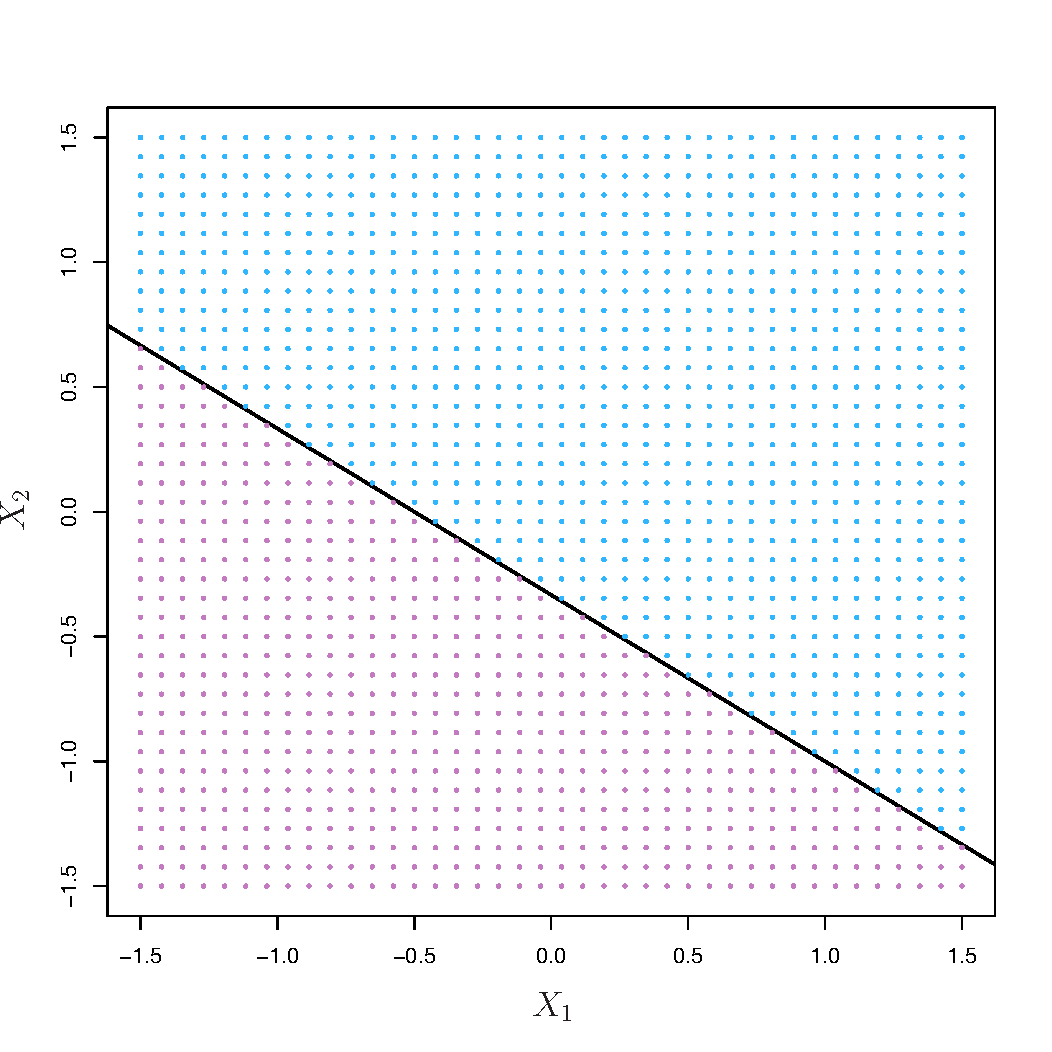
\includegraphics[scale=0.30]{9-1.pdf}
        \caption{(Figura 9.1 de [ISLP]) Hiperplano $1 + 2x_1 + 3x_2 = 0$ em $\RR^2$ (linha sólida). A região azul são os pontos $\V{x}$ tais que $1 + 2x_1 + 3x_2 > 0$ e região roxa são os pontos $\V{x}$ tais que $1 + 2x_1 + 3x_2 < 0$.}
    \end{figure}
\end{frame}

%%%%%%%%%%%%%%%%%%%%%%%%%%%%%%%%%%%%%%%%%%%

%%%%%%%%%%%%%%%%%%%%%%%%%%%%%%%%%%%%%%%%%%%

\begin{frame}{Classificador de margem máxima -- construção}
    \begin{itemize}
        \item Matriz $\V{X}_{n \times p}$ de $n$ observações em $\RR^p$: $$\V{X} = \begin{bmatrix} - & \V{x}_1^T & - \\
         & \vdots & \\
        - & \V{x}_n^T & - \end{bmatrix} = \begin{bmatrix} x_{11} & \dots & x_{1p} \\
        \vdots & \ddots & \vdots \\
        x_{n1} & \dots & x_{np} \end{bmatrix}$$
        
        \pause
        
        \item Observações em duas classes: $y_1, \dots, y_n \in \{-1, 1\}$
        
        \pause
        
        \item Nova observação $\V{x}^* = (x_1^*, \dots, x_p^*)^T$ que desejamos classificar
        
        \pause
        
        \item Assuma que as classes sejam linearmente separáveis
    \end{itemize}
    
    \pause
    
    \begin{center}
        $\implies$ Como escolher o ``melhor"~hiperplano classificador?
    \end{center}
\end{frame}

%%%%%%%%%%%%%%%%%%%%%%%%%%%%%%%%%%%%%%%%%%%

%%%%%%%%%%%%%%%%%%%%%%%%%%%%%%%%%%%%%%%%%%%

\begin{frame}{Classificador de margem máxima -- construção}
    \begin{figure}
        \center
        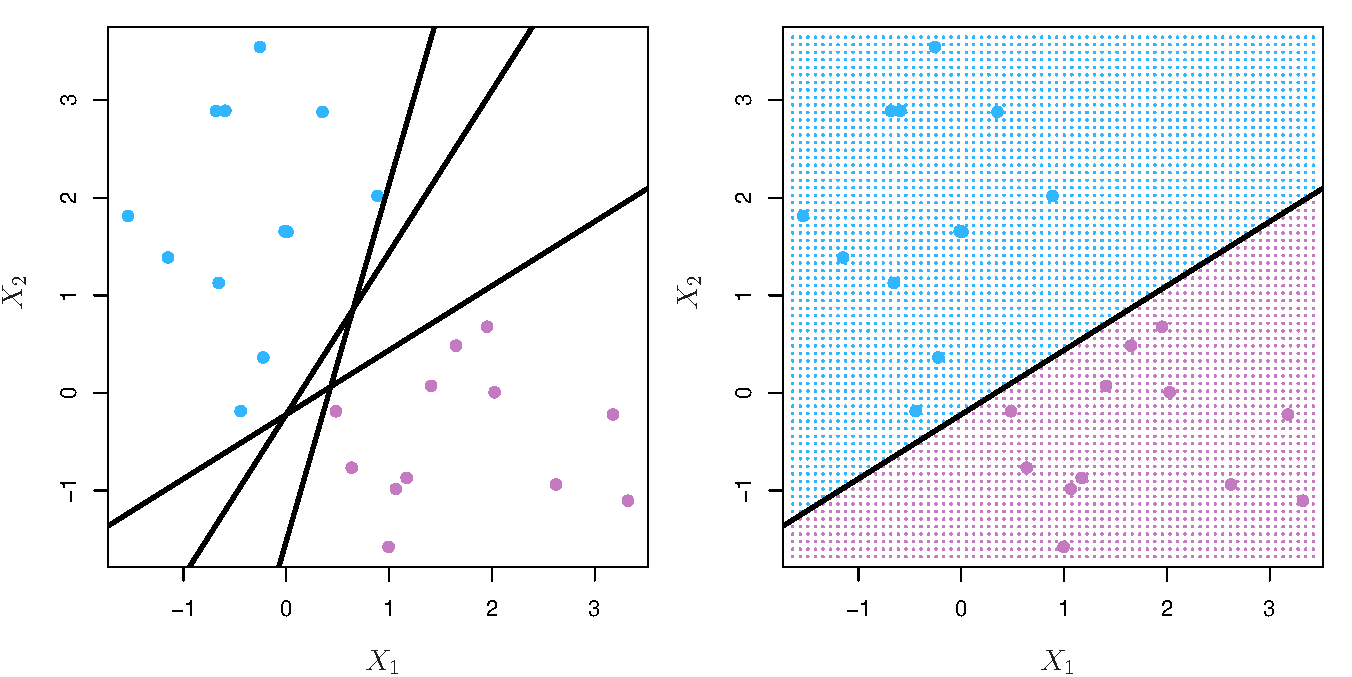
\includegraphics[scale=0.43]{9-2.pdf}
        \caption{(Figura 9.2 de [ISLP]) Esquerda: Duas classes e três hiperplanos separadores. Direita: Um hiperplano separador e sua respectiva regra de decisão.}
    \end{figure}
\end{frame}

%%%%%%%%%%%%%%%%%%%%%%%%%%%%%%%%%%%%%%%%%%%

%%%%%%%%%%%%%%%%%%%%%%%%%%%%%%%%%%%%%%%%%%%

\begin{frame}{Classificador de margem máxima -- construção}
    \begin{itemize}
        \item Azul  $\iff y_i = 1$ e roxo $\iff y_i = -1$
        
        \pause
        
        \item Um hiperplano separador satisfaz $$\beta_0 + \beta_1 x_{i1} + \dots + \beta_p x_{ip} > 0 \text{ se } y_i = 1$$
        $$\beta_0 + \beta_1 x_{i1} + \dots + \beta_p x_{ip} < 0 \text{ se } y_i = -1$$
        
        \pause
        
        \item Equivalentemente, $$y_i(\beta_0 + \beta_1 x_{i1} + \dots + \beta_p x_{ip}) > 0, \forall i = 1, \dots, n$$
        
        \pause
        
        \item $\implies$ Podemos construir um classificador com base no \alert{sinal} de $f(\V{x}^*) = \beta_0 + \beta_1 x_1^* + \dots + \beta_p x_p^*$...
        
        \pause
        
        \item ...e a \alert{magnitude} de $f(\V{x}^*)$ nos dá a ``distância"~ao hiperplano (confiança na classificação)
    \end{itemize}
\end{frame}

%%%%%%%%%%%%%%%%%%%%%%%%%%%%%%%%%%%%%%%%%%%

%%%%%%%%%%%%%%%%%%%%%%%%%%%%%%%%%%%%%%%%%%%

\begin{frame}{Classificador de margem máxima -- construção}
    \begin{itemize}
        \item Dados linearmente separáveis $\implies$ falta de unicidade no hiperplano separador!
        
        \pause
        
        \item Solução: escolher aquele que esteja mais longe das observações de treinamento!
        
        \pause
        
        \begin{itemize}
            \item Distância de cada observação de treinamento a um dado hiperplano
            
            \pause
            
            \item Menor dessas distâncias: \alert{margem} do hiperplano
            
            \pause
            
            \item Escolher o hiperplano de maior margem -- aquele que tem maior distância mínima às observações de treinamento
            
            \pause
            
            \item Daí o nome do classificador!
        \end{itemize}
        
        \pause
        
        \item No classificador de margem máxima, as observações que atingem a margem são chamados de \alert{vetores suporte}
    \end{itemize}
\end{frame}

%%%%%%%%%%%%%%%%%%%%%%%%%%%%%%%%%%%%%%%%%%%

%%%%%%%%%%%%%%%%%%%%%%%%%%%%%%%%%%%%%%%%%%%

\begin{frame}{Classificador de margem máxima -- construção}
    \begin{figure}
        \center
        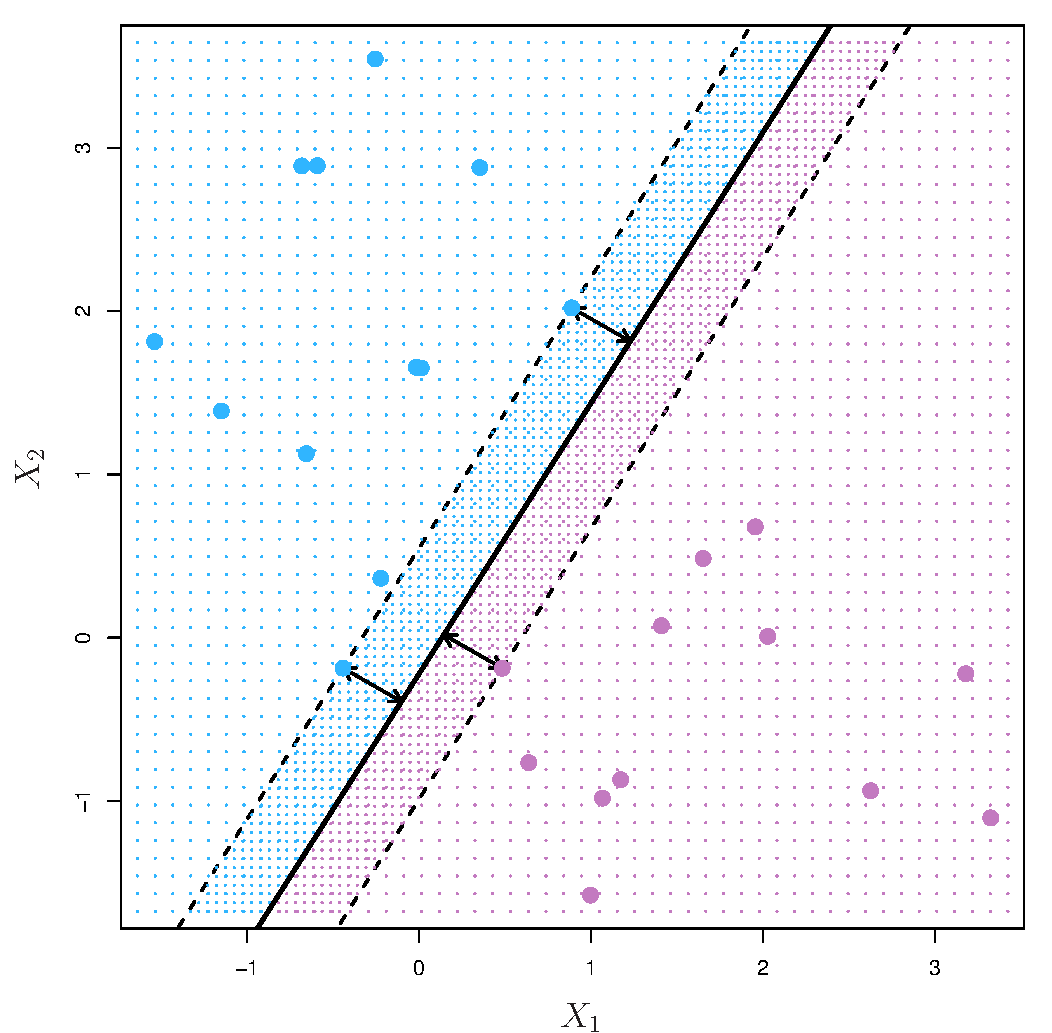
\includegraphics[scale=0.25]{9-3.pdf}
        \caption{(Figura 9.2 de [ISLP]) Classificador de margem máxima (linha sólida), margens (linhas tracejadas) e os respectivos vetores suporte.}
    \end{figure}
    
    \pause
    
    \begin{center}
        $\implies$ O classificador de margem máxima depende somente dos vetores suporte, e não das outras observações!
    \end{center}
\end{frame}

%%%%%%%%%%%%%%%%%%%%%%%%%%%%%%%%%%%%%%%%%%%

%%%%%%%%%%%%%%%%%%%%%%%%%%%%%%%%%%%%%%%%%%%

\begin{frame}{Classificador de margem máxima -- construção}
    \textbf{Definição}: O classificador de margem máxima, sob a hipótese de classes linearmente separáveis, é a solução do seguinte problema de otimização:
    \begin{align*}
        &\max_{\beta_0, \beta_1, \dots, \beta_p, M} M  ~~~~ (\star) \\ 
        &\text{sujeito a } \sum_{j = 1}^{p} \beta_j^2 = 1 ~~~~ (\star \star)\\
        &\text{e } y_i(\beta_0 + \beta_1 x_{i1} + \dots + \beta_p x_{ip}) \geq M, \forall i = 1, \dots, n ~~~~ (\star \star \star)
    \end{align*}
    
    \pause
    
    \begin{itemize}
        \item $(\star \star \star)$: Todas as observações estão do lado ``certo"~do hiperplano, com uma ``gordurinha"~$M > 0$
        
        \pause
        
        \item $(\star \star)$: Unicidade na fórmula do hiperplano de margem máxima
    \end{itemize}
    
    \pause
    
    \begin{center}
        $\implies$ Se as classes não são linearmente separáveis, o problema de otimização $(\star, \star \star, \star \star \star)$ não tem solução com $M > 0$!
    \end{center}
\end{frame}

%%%%%%%%%%%%%%%%%%%%%%%%%%%%%%%%%%%%%%%%%%%

%%%%%%%%%%%%%%%%%%%%%%%%%%%%%%%%%%%%%%%%%%%

\begin{frame}{Classificador de margem máxima -- limitação}
    \begin{figure}
        \center
        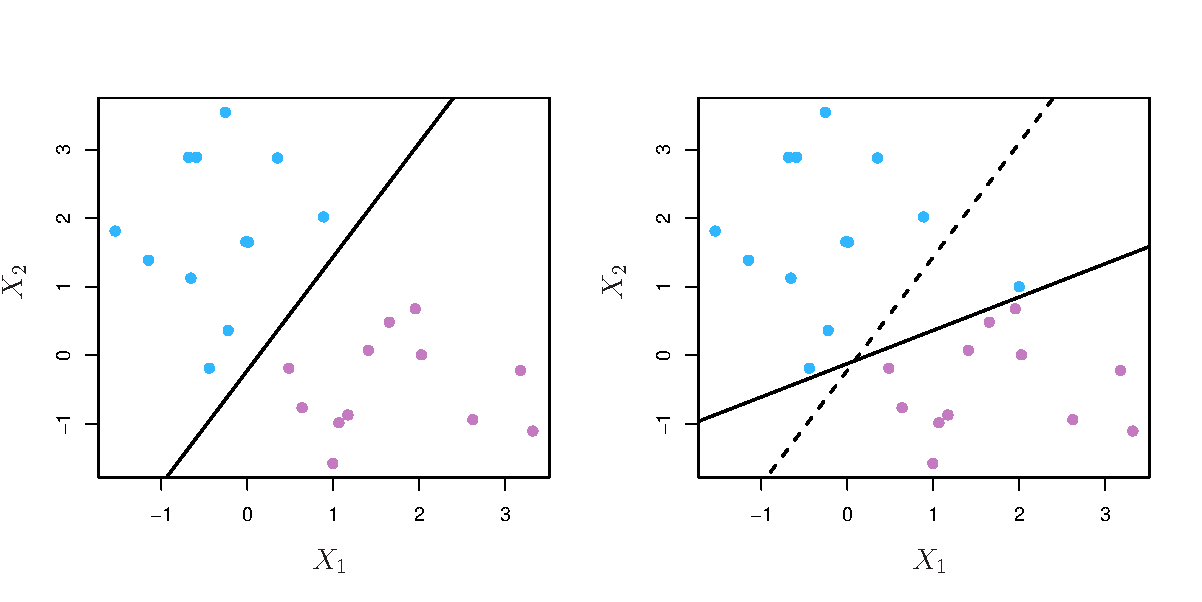
\includegraphics[scale=0.40]{9-5.pdf}
        \caption{(Figura 9.5 de [ISLP]) Esquerda: Classificador de margem máxima. Direita: Classificadores de margem máxima antigo (linha pontilhada) e novo (linha sólida) após acrescentar uma nova observação no conjunto de treinamento.}
    \end{figure}
    
    \pause
    
    \begin{center}
        $\implies$ Alta sensibilidade a novas observações, possível sobreajuste!
    \end{center}
\end{frame}

%%%%%%%%%%%%%%%%%%%%%%%%%%%%%%%%%%%%%%%%%%%

%%%%%%%%%%%%%%%%%%%%%%%%%%%%%%%%%%%%%%%%%%%

\begin{frame}{Classificador de vetor suporte -- motivação}
    \begin{itemize}
        \item Pode valer a pena classificar errado algumas observações em prol de:
        \begin{itemize}
            \item Maior robustez a observações individuais
            
            \item Classificação mais \alert{confiável} (i.e., mais distante do hiperplano separador) da \textit{maioria} das observações
        \end{itemize}
    \end{itemize}
    
    \pause
    
    \begin{center}
        $\implies$ Em vez de exigir que \alert{todas} as observações estejam do lado ``certo"~da margem, permitir que algumas estejam do lado ``errado"~da margem, talvez até do lado ``errado"~do hiperplano!
    \end{center}
    
    \pause
    
    \textbf{Observação}: Além de resolver os dois problemas acima, resolve o problema das classes não serem linearmente separáveis
\end{frame}

%%%%%%%%%%%%%%%%%%%%%%%%%%%%%%%%%%%%%%%%%%%

%%%%%%%%%%%%%%%%%%%%%%%%%%%%%%%%%%%%%%%%%%%

\begin{frame}{Classificador de vetor suporte -- motivação}
    \begin{figure}
        \center
        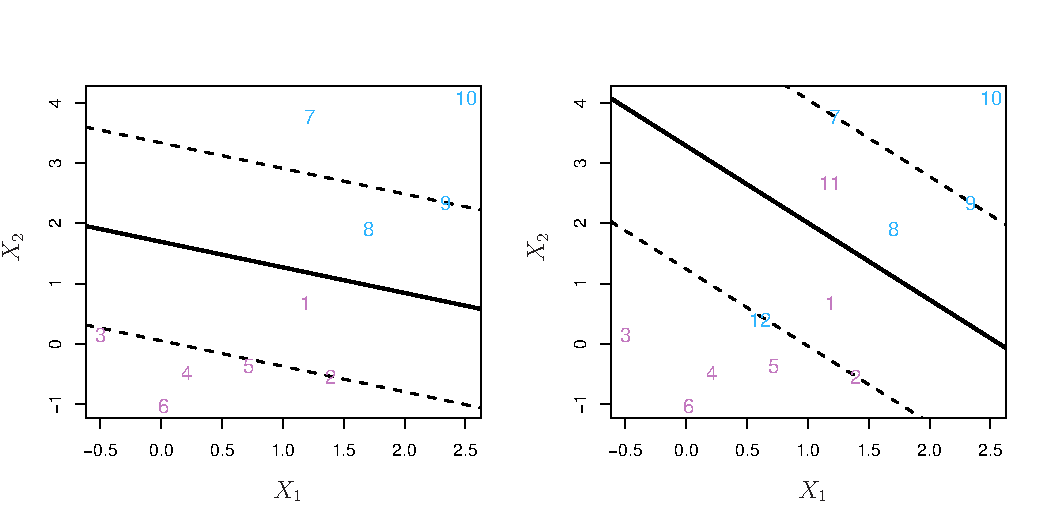
\includegraphics[scale=0.55]{9-6.pdf}
        \caption{(Figura 9.6 de [ISLP]) Hiperplanos de margem máxima (linha sólida) e margens (linhas tracejadas). Esquerda: Algumas observações do lado ``errado"~da margem, porém nenhuma do lado ``errado"~do hiperplano. Direita: Observações do lado ``errado"~da margem e do hiperplano, após acréscimo de duas novas observações, 11 e 12.}
    \end{figure}
\end{frame}

%%%%%%%%%%%%%%%%%%%%%%%%%%%%%%%%%%%%%%%%%%%

%%%%%%%%%%%%%%%%%%%%%%%%%%%%%%%%%%%%%%%%%%%

\begin{frame}{Classificador de vetor suporte -- construção}
    \textbf{Definição}: O classificador de vetor suporte é a solução do seguinte problema de otimização:
    \begin{align*}
        &\max_{\beta_0, \beta_1, \dots, \beta_p, \alert{\varepsilon_1, \dots, \varepsilon_n}, M} M  ~~~~ (*) \\ 
        &\text{sujeito a } \sum_{j = 1}^{p} \beta_j^2 = 1 ~~~~ (**)\\
        &y_i(\beta_0 + \beta_1 x_{i1} + \dots + \beta_p x_{ip}) \geq M\alert{(1 - \varepsilon_i)}, \forall i = 1, \dots, n ~~~~ (***) \\
        &\alert{\varepsilon_i \geq 0 \text{ e } \sum_{i = 1}^{n} \varepsilon_i \leq C} ~~~~ (****)
    \end{align*}
    
    \pause
    
    \begin{itemize}
        \item $\varepsilon_i = 0 \iff$ observação $i$ do lado ``certo"~do hiperplano
        
        \item $\varepsilon_i > 1 \iff$ observação $i$ do lado ``errado"~do hiperplano
        
        \item $0 < \varepsilon_i < 1 \iff$ observação $i$ do lado ``certo"~do hiperplano porém do lado ``errado"~da margem
    \end{itemize}
\end{frame}

%%%%%%%%%%%%%%%%%%%%%%%%%%%%%%%%%%%%%%%%%%%

%%%%%%%%%%%%%%%%%%%%%%%%%%%%%%%%%%%%%%%%%%%

\begin{frame}{Classificador de vetor suporte -- análise}
    \begin{itemize}
        \item $(****)$: $\ds \sum_{i = 1}^{n} \varepsilon_i \leq C \iff C$ representa um \alert{orçamento} para as violações do hiperplano:
        
        \pause
        
        \begin{itemize}
            \item $C = 0$ reduz ao caso do classificador de margem máxima: nenhuma violação é permitida ($\varepsilon_1 = \dots = \varepsilon_n = 0$)
            
            \pause
            
            \item $C > 0 \iff$ não mais que $C$ observações podem estar classificadas erroneamente, no pior dos casos
        \end{itemize}
        
        \pause
        
        \item $\uparrow C \implies$ mais tolerantes com classificações errôneas $\implies$ maior margem $\implies$ $\uparrow$ viés e $\downarrow$ variância
        
        \pause
        
        \item $\downarrow C \implies$ menos tolerantes com classificações errôneas $\implies$ menor margem $\implies$ $\downarrow$ viés e $\uparrow$ variância
        
        \pause
        
        \item Escolher $C$ através de validação cruzada, por exemplo
    \end{itemize}
\end{frame}

%%%%%%%%%%%%%%%%%%%%%%%%%%%%%%%%%%%%%%%%%%%

%%%%%%%%%%%%%%%%%%%%%%%%%%%%%%%%%%%%%%%%%%%

\begin{frame}{Classificador de vetor suporte -- análise}
    \begin{figure}
        \center
        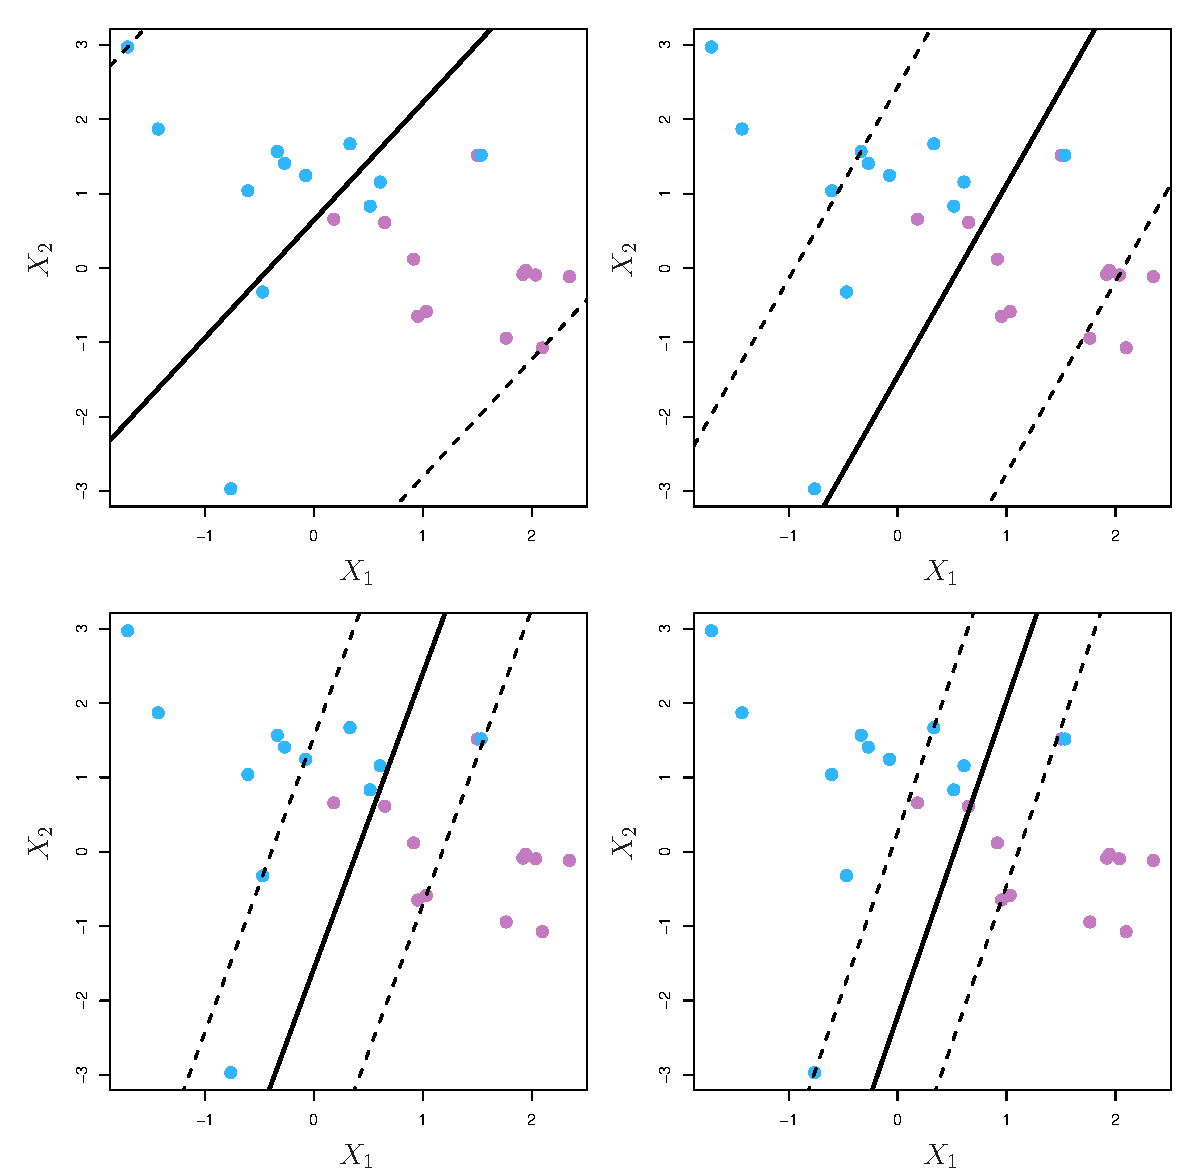
\includegraphics[scale=0.30]{9-7.pdf}
        \caption{(Figura 9.7 de [ISLP]) Classificadores de vetor suporte ajustados com quatro valores de $C$ distintos. Hiperplanos separadores em linha sólida e margens em linha pontilhada.}
    \end{figure}
\end{frame}

%%%%%%%%%%%%%%%%%%%%%%%%%%%%%%%%%%%%%%%%%%%

%%%%%%%%%%%%%%%%%%%%%%%%%%%%%%%%%%%%%%%%%%%

\begin{frame}{Classificador de vetor suporte -- análise}
    \begin{itemize}
        \item O hiperplano depende somente das observações que estão do lado ``errado"~da margem e do hiperplano $\implies$ \alert{vetores suporte}
        
        \pause
        
        \item De acordo com o balanço entre viés e variância:
        \begin{itemize}
            \item $\uparrow C \implies$ margem larga $\implies$ mais vetores suporte $\implies$ $\downarrow$ variância
            
            \pause
            
            \item $\downarrow C \implies$ margem estreita $\implies$ menos vetores suporte $\implies$ \\ $\uparrow$ variância
        \end{itemize}
    \end{itemize}
    
    \pause
    
    \begin{center}
        $\implies$ Insensibilidade a observações ``longe"~do hiperplano separador!
    \end{center}
    
    \pause
    
    \textbf{Observação}: Distinto de outros métodos com fronteira de decisão lineares!
    
    \pause
    
    \begin{itemize}
        \item LDA depende (e é sensível) a todas as observações
        
        \pause
        
        \item Regressão logística é pouco sensível a observações ``longe"~da fronteira de decisão
    \end{itemize}
\end{frame}

%%%%%%%%%%%%%%%%%%%%%%%%%%%%%%%%%%%%%%%%%%%

%%%%%%%%%%%%%%%%%%%%%%%%%%%%%%%%%%%%%%%%%%%

\begin{frame}{Classificador de vetor suporte -- observação importante}
    \textbf{Observação}: O que é resolvido numericamente \alert{não} são as equações $(*, **, ***, ****)$, mas sim:
    $$\min_{\substack{\beta_0, \beta_1, \dots, \beta_p, \\ \varepsilon_1, \dots, \varepsilon_n}} \|(\beta_1, \dots, \beta_p)\|_2 \text{ t.q. } \begin{cases} y_i(\beta_0 + \beta_1 x_{i1} + \dots + \beta_p x_{ip}) \geq 1 - \varepsilon_i \\ \varepsilon_i \geq 0, \sum_{i = 1}^{n} \varepsilon_i \leq C, \forall i = 1, \dots, n\end{cases}$$
    
    \pause
    
    \begin{center}
        $\implies$ Problema quadrático com restrições lineares $\implies$ problema de otimização convexa!
    \end{center}
    
    \pause
    
    Equivalente a resolver o problema (multiplicadores de Lagrange):
    $$\min_{\substack{\beta_0, \beta_1, \dots, \beta_p, \\ \varepsilon_1, \dots, \varepsilon_n}} \frac{1}{2}\|(\beta_1, \dots, \beta_p)\|_2^2 + C\sum_{i = 1}^{n} \varepsilon_i, \text{ t.q. } \varepsilon_i \geq 0$$ $$\text{e } y_i(\beta_0 + \beta_1 x_{i1} + \dots + \beta_p x_{ip}) \geq 1 - \varepsilon_i, \forall i = 1, \dots, n$$

\end{frame}

%%%%%%%%%%%%%%%%%%%%%%%%%%%%%%%%%%%%%%%%%%%

%%%%%%%%%%%%%%%%%%%%%%%%%%%%%%%%%%%%%%%%%%%

\begin{frame}{Cuidado: o $C$ do slide anterior aparece de duas formas}
    Repare que a \alert{mesma letra} foi usada para dois papéis \alert{opostos}:

    \pause

    \begin{itemize}
        \item em $(****)$, $\ds \sum_{i = 1}^{n} \varepsilon_i \leq C$: o $C$ é o \alert{orçamento} de violações. É a convenção do [ISLP] e do [AME] --- a dos slides anteriores;

        \pause

        \item na forma de Lagrange, $\ds \frac{1}{2}\|(\beta_1, \dots, \beta_p)\|_2^2 + C\sum_{i = 1}^{n} \varepsilon_i$: o $C$ é o \alert{peso da penalidade} sobre as violações --- e é esta a convenção do \texttt{scikit-learn}
    \end{itemize}

    \pause

    \begin{center}
        $\implies$ Tudo o que dissemos sobre ``$\uparrow C$'' se \alert{inverte} de uma para a outra!
    \end{center}

    \pause

    No \texttt{scikit-learn}: $\uparrow C \implies$ penaliza mais $\implies$ tolera menos $\implies$ margem \alert{estreita} $\implies$ \alert{menos} vetores suporte.
\end{frame}

%%%%%%%%%%%%%%%%%%%%%%%%%%%%%%%%%%%%%%%%%%%

%%%%%%%%%%%%%%%%%%%%%%%%%%%%%%%%%%%%%%%%%%%

\begin{frame}{Cuidado: o $C$ do slide anterior aparece de duas formas}
    E não é sutileza de notação --- dá para medir. Na Seção 8 da \texttt{Aula prática 09}, ajustando \texttt{SVC} ao \texttt{breast\_cancer} com $\gamma$ e \emph{kernel} fixos:

    \pause

    \begin{center}\small
    \renewcommand{\arraystretch}{1.3}
    \begin{tabular}{@{}lrrr@{}}
    \toprule
     & vetores suporte & \% do treino & AUC no teste \\
    \midrule
    \texttt{SVC(C=0.01)} & $92$ & $23{,}1\%$ & $0{,}9921$ \\
    \texttt{SVC(C=1000)} & $24$ & $6{,}0\%$ & $0{,}9911$ \\
    \bottomrule
    \end{tabular}
    \end{center}

    \pause

    O $C$ \emph{pequeno} do \texttt{scikit-learn} é que dá \alert{mais} vetores suporte --- quatro vezes mais --- exatamente ao contrário do que os slides anteriores dizem do $C$ deles.

    \pause

    \begin{center}
        $\implies$ Ao ler qualquer texto sobre SVM, confira \alert{qual} $C$ está em uso antes de interpretar ``$C$ grande''!
    \end{center}
\end{frame}

%%%%%%%%%%%%%%%%%%%%%%%%%%%%%%%%%%%%%%%%%%%

%%%%%%%%%%%%%%%%%%%%%%%%%%%%%%%%%%%%%%%%%%%

% \setcounter{framenumber}{0}
% \set\date{Aula 22}

%%%%%%%%%%%%%%%%%%%%%%%%%%%%%%%%%%%%%%%%%%%

%%%%%%%%%%%%%%%%%%%%%%%%%%%%%%%%%%%%%%%%%%%

\begin{frame}{Classificador de vetor suporte -- limitação}
    \begin{figure}
        \center
        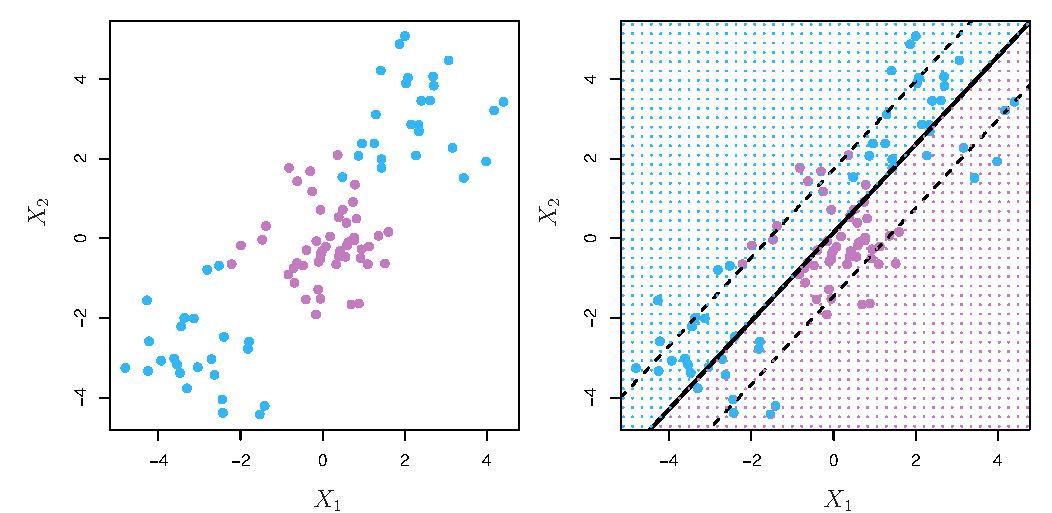
\includegraphics[scale=0.60]{9-8.pdf}
        \caption{(Figura 9.8 de [ISLP]) Esquerda: Observações em duas classes. Direita: Tentativa de ajustar um classificador de vetor suporte a tal conjunto de dados.}
    \end{figure}
\end{frame}

%%%%%%%%%%%%%%%%%%%%%%%%%%%%%%%%%%%%%%%%%%%

%%%%%%%%%%%%%%%%%%%%%%%%%%%%%%%%%%%%%%%%%%%

\begin{frame}{Máquina de vetores suporte (SVM) -- primeira ideia}
    Lembremos do classificador de vetor suporte:
    \begin{align*}
        &\max_{\beta_0, \beta_1, \dots, \beta_p, \varepsilon_1, \dots, \varepsilon_n, M} M \\ 
        &\text{sujeito a } \sum_{j = 1}^{p} \beta_j^2 = 1 \\
        &y_i(\beta_0 + \beta_1 x_{i1} + \dots + \beta_p x_{ip}) \geq M(1 - \varepsilon_i), \forall i = 1, \dots, n \\
        &\varepsilon_i \geq 0 \text{ e } \sum_{i = 1}^{n} \varepsilon_i \leq C
    \end{align*}
    
    \pause
    
    \begin{center}
        $\implies$ Em vez de ajustar o classificador com $X_1, \dots, X_p$, acrescentar também $X_1^2, \dots, X_p^2$!
    \end{center}
\end{frame}

%%%%%%%%%%%%%%%%%%%%%%%%%%%%%%%%%%%%%%%%%%%

%%%%%%%%%%%%%%%%%%%%%%%%%%%%%%%%%%%%%%%%%%%

\begin{frame}{Máquina de vetores suporte (SVM) -- primeira ideia}
    \vspace{-0.7cm}
    \begin{align*}
        &\max_{\beta_0, \beta_{11}, \dots, \beta_{p1}, \alert{\beta_{12}, \dots, \beta_{p2}}, \varepsilon_1, \dots, \varepsilon_n, M} M \\ 
        &\text{sujeito a }\alert{\sum_{j = 1}^{p}\sum_{k = 1}^{2} \beta_{jk}^2 = 1}, \varepsilon_i \geq 0 \text{ e } \sum_{i = 1}^{n} \varepsilon_i \leq C \\
        &y_i\left(\beta_0 + \sum_{j = 1}^{p} \beta_{j1} x_{ij} + \alert{\sum_{j = 1}^{p} \beta_{j2} x_{ij}^2}\right) \geq M(1 - \varepsilon_i), \forall i = 1, \dots, n
    \end{align*}
    
    \pause
    
    \begin{itemize}
        \item No espaço aumentado $X_1, \dots, X_p, X_1^2, \dots, X_p^2$ $\implies$ fronteira de decisão linear
        
        \pause
        
        \item No espaço original $X_1, \dots, X_p$ $\implies$ fronteira de decisão quadrática
        
        \pause
        
        \item Quantidade de coeficientes a estimar aumenta muito! $\implies$ baixa eficiência computacional
    \end{itemize}
    
    \pause
    
    \begin{center}
        Podemos tornar os dados separáveis em um espaço de dimensão infinita sem aumentar a quantidade de parâmetros a estimar!
    \end{center}
\end{frame}

%%%%%%%%%%%%%%%%%%%%%%%%%%%%%%%%%%%%%%%%%%%

%%%%%%%%%%%%%%%%%%%%%%%%%%%%%%%%%%%%%%%%%%%

\begin{frame}{Máquina de vetores suporte (SVM) -- construção}
    Podemos mostrar que:
    \begin{itemize}
        \item A fronteira de decisão do classificador de vetor suporte pode ser escrita como $$f(\V{x}) = \beta_0 + \sum_{i = 1}^{n} \alpha_i \langle \V{x}, \V{x}_i\rangle,$$ onde $\V{x}_1, \dots, \V{x}_n$, são as observações de treinamento
        
        \pause
        
        \item Para estimar $\beta_0, \alpha_1, \dots, \alpha_n$ precisamos somente dos $\ds \binom{n}{2}$ produtos internos $\langle \V{x}_i, \V{x}_j \rangle$, para $1 \leq i < j \leq n$
        
        \pause
        
        \item Os únicos $\alpha_i \neq 0$ são os referentes aos vetores suporte: \pause $$f(\V{x}) = \beta_0 + \sum_{i \in \mathcal{S}} \alpha_i \langle \V{x}, \V{x}_i\rangle,$$ onde $\mathcal{S}$ é o conjunto dos índices dos vetores suporte
    \end{itemize}
    
    \pause
    
    \begin{center}
        $\implies$ Calcular e estimar $f$ só precisa de produtos internos!
    \end{center}
\end{frame}

%%%%%%%%%%%%%%%%%%%%%%%%%%%%%%%%%%%%%%%%%%%

%%%%%%%%%%%%%%%%%%%%%%%%%%%%%%%%%%%%%%%%%%%

\begin{frame}{Digressão de Álgebra Linear}
    \begin{itemize}
        \item O produto interno $\langle \V{x}, \V{y} \rangle$ mede \alert{similaridade} entre os vetores $\V{x}, \V{y} \in \RR^p$
        
        \pause
        
        \item Como podemos medir similaridade de outras formas?
        
        \pause
        
        \begin{itemize}
            \item $k: \RR^p \times \RR^p \to \RR \implies k(\V{x}, \V{y})$ generalização de $\langle \cdot, \cdot \rangle: \RR^p \times \RR^p \to \RR$, dito um \alert{\textit{kernel}}
            
            \pause
            
            \item $\ds k(\V{x}, \V{y}) = \left(1 + \sum_{j = 1}^{p} x_j y_j \right)^d$, \textit{kernel} polinomial de grau $d$
            
            \pause
            
            \item $\ds k(\V{x}, \V{y}) = \exp\left(-\gamma \sum_{j = 1}^{p} (x_j - y_j)^2 \right)$, \textit{kernel} radial ou exponencial quadrático
            
            \pause
            
            \item Obviamente $k(\V{x}, \V{y}) = \langle \V{x}, \V{y} \rangle$! \textit{Kernel} linear
            
            \pause
            
            \item ... muitos outros!
        \end{itemize}
    \end{itemize}
\end{frame}

%%%%%%%%%%%%%%%%%%%%%%%%%%%%%%%%%%%%%%%%%%%

%%%%%%%%%%%%%%%%%%%%%%%%%%%%%%%%%%%%%%%%%%%

\begin{frame}{Digressão de Álgebra Linear}
    \begin{center}
        Mas quais funções $k:\RR^p \times \RR^p \to \RR$ são ``boas"~para medir similaridade entre dois vetores?
    \end{center}
    
    \pause
    
    \textbf{Resposta}: Devem existir $\Hcal$ espaço de Hilbert e $\varphi: \RR^p \to \Hcal$ tais que $$k(\V{x}, \V{y}) = \langle \varphi(\V{x}), \varphi(\V{y}) \rangle_{\Hcal}$$
    
    \pause
    
    \begin{center}
        $\implies$ Intuitivamente, os dados devem ser linearmente separáveis em algum espaço, potencialmente de dimensão infinita.
    \end{center}
    
    \pause
    
    \textbf{Teorema}: A função $k:\RR^p \times \RR^p \to \RR$ é um \textit{kernel} (i.e., existem $\Hcal$ e $\varphi$ como acima) se e somente se ela é positiva semidefinida: $$\int_{\RR^p} \int_{\RR^p} g(\V{x}) k(\V{x}, \V{y}) g(\V{y})~d\V{x}d\V{y} \geq 0,$$ para toda $g: \RR^p \to \RR$ tal que $\int_{\RR^p} \|g(\V{x})\|^2~d\V{x} < \infty$.
\end{frame}

%%%%%%%%%%%%%%%%%%%%%%%%%%%%%%%%%%%%%%%%%%%

%%%%%%%%%%%%%%%%%%%%%%%%%%%%%%%%%%%%%%%%%%%

\begin{frame}{Digressão de Álgebra Linear}
    \begin{figure}
        \center
        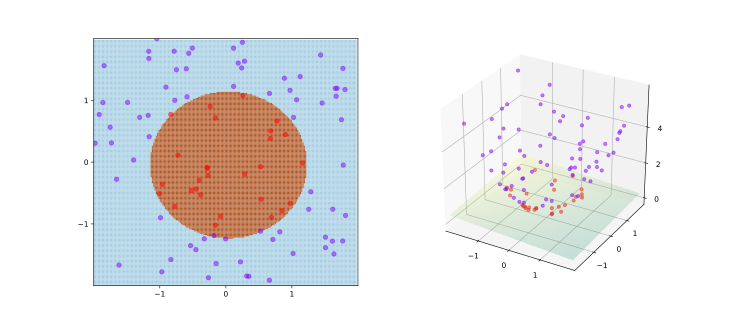
\includegraphics[scale=0.50]{kernel-trick.png}
        \caption{[Wikipedia] $\varphi: \RR^2 \to \RR^3$ dada por $\varphi(x_1, x_2) = (x_1, x_2, x_1^2 + x_2^2)$ e portanto $k(\V{x}, \V{y}) = \langle \V{x}, \V{y} \rangle + \|\V{x}\|^2\|\V{y}\|^2$. Dados não-separáveis linearmente em $\RR^2$ mas sim em $\RR^3$.}
    \end{figure}
\end{frame}

%%%%%%%%%%%%%%%%%%%%%%%%%%%%%%%%%%%%%%%%%%%

%%%%%%%%%%%%%%%%%%%%%%%%%%%%%%%%%%%%%%%%%%%

\begin{frame}{Máquina de vetores suporte (SVM) -- construção}
    \begin{itemize}
        \item Escolha o seu \textit{kernel} preferido $k$
        
        \pause
        
        \item Encontre a fronteira de decisão da forma $\ds f(\V{x}) = \beta_0 + \sum_{i \in \mathcal{S}} \alpha_i k(\V{x}, \V{x}_i)$
    \end{itemize}
    
    \pause
    
    \begin{center}
        $\implies$ Eis o SVM!
    \end{center}
    
    \pause
    
    \begin{figure}
        \center
        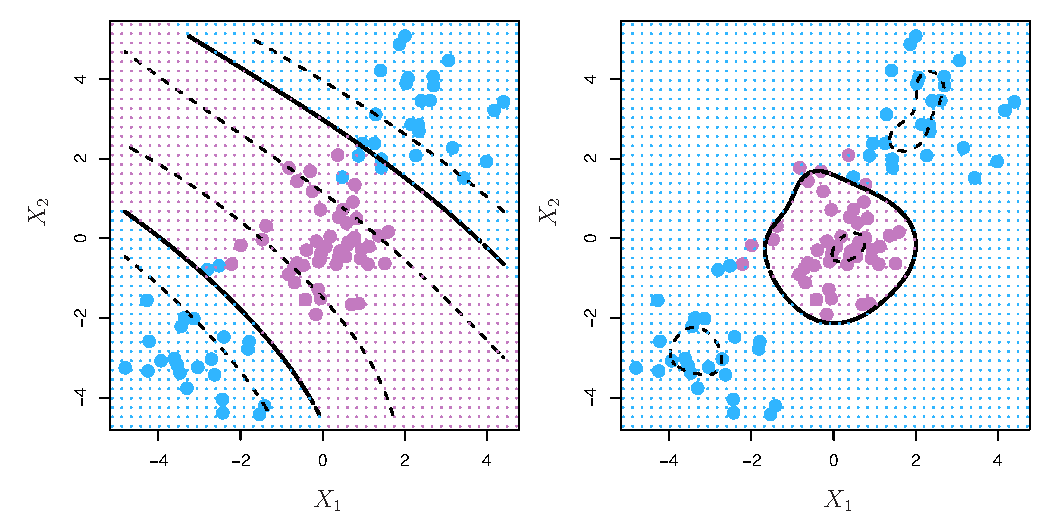
\includegraphics[scale=0.45]{9-9.pdf}
        \caption{(Figura 9.9 de [ISLP]) Esquerda: Ajuste com \textit{kernel} polinomial de grau 3. Direita: Ajuste com \textit{kernel} radial.}
    \end{figure}
\end{frame}

%%%%%%%%%%%%%%%%%%%%%%%%%%%%%%%%%%%%%%%%%%%

%%%%%%%%%%%%%%%%%%%%%%%%%%%%%%%%%%%%%%%%%%%

\begin{frame}{Relação com regressão logística}
    Lembremos do classificador de vetor suporte (caso particular do SVM com \textit{kernel} linear:
    \begin{align*}
        &\max_{\beta_0, \beta_1, \dots, \beta_p, \varepsilon_1, \dots, \varepsilon_n, M} M \\ 
        &\text{sujeito a } \sum_{j = 1}^{p} \beta_j^2 = 1, \varepsilon_i \geq 0 \text{ e } \sum_{i = 1}^{n} \varepsilon_i \leq C \\
        &y_i(\beta_0 + \beta_1 x_{i1} + \dots + \beta_p x_{ip}) \geq M(1 - \varepsilon_i), \forall i = 1, \dots, n
    \end{align*}
    
    \pause
    
    Esse problema de otimização pode ser escrito como $$\min_{\beta_0, \beta_1, \dots, \beta_p} \left\{\sum_{i = 1}^{n} \max[0, 1 - y_i f(\V{x}_i)] + \lambda \sum_{j = 1}^{p} \beta_j^2\right\},$$ onde $f(\V{x}) = \beta_0 + \beta_1 x_1 + \dots + \beta_p x_p$
\end{frame}

%%%%%%%%%%%%%%%%%%%%%%%%%%%%%%%%%%%%%%%%%%%

%%%%%%%%%%%%%%%%%%%%%%%%%%%%%%%%%%%%%%%%%%%

\begin{frame}{Relação com regressão logística}
    $$\min_{\beta_0, \beta_1, \dots, \beta_p} \left\{\sum_{i = 1}^{n} \max[0, 1 - y_i f(\V{x}_i)] + \lambda \sum_{j = 1}^{p} \beta_j^2\right\}$$
    
    \pause
    
    $$\Downarrow$$
    
    $$\min_{\beta_0, \beta_1, \dots, \beta_p} \left\{L(\V{X}, \V{y}, \Vg{\beta}) + \lambda P(\Vg{\beta})\right\},$$ onde $L$ é uma \alert{função custo} e $P$ é uma \alert{penalidade}
    
    \pause
    
    \begin{itemize}
        \item A função custo mede o ajuste do modelo aos dados
        
        \item A penalidade impõe uma restrição desejada \textit{a priori} no modelo
        
        \pause
        
        \item O modelo de regressão logística também pode ser escrito nessa forma
    \end{itemize}
\end{frame}

%%%%%%%%%%%%%%%%%%%%%%%%%%%%%%%%%%%%%%%%%%%

%%%%%%%%%%%%%%%%%%%%%%%%%%%%%%%%%%%%%%%%%%%

\begin{frame}{Relação com regressão logística}
    \begin{figure}
        \center
        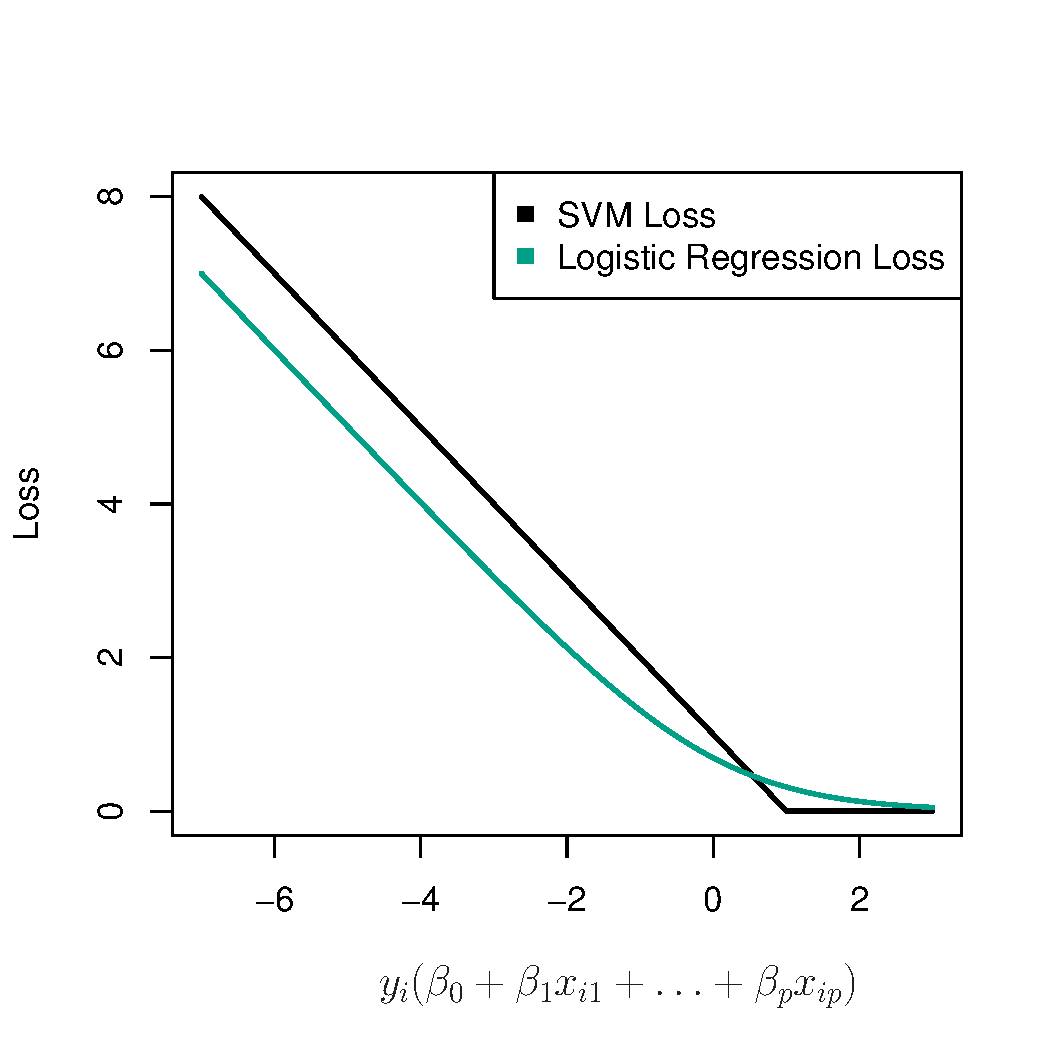
\includegraphics[scale=0.32]{9-12.pdf}
        \caption{(Figura 9.12 de [ISLP]) Funções perda associadas à regressão logística (verde) e classificador de vetor suporte (preto), como função de $y_i(\beta_0 + \beta_1 x_{i1} + \dots + \beta_p x_{ip})$.}
    \end{figure}
\end{frame}

%%%%%%%%%%%%%%%%%%%%%%%%%%%%%%%%%%%%%%%%%%%

%%%%%%%%%%%%%%%%%%%%%%%%%%%%%%%%%%%%%%%%%%%

\begin{frame}{Relação com regressão logística}
    \begin{itemize}
        \item Na formulação de custo + penalidade, a margem do classificador de vetor suporte corresponde ao valor 1, e o seu tamanho é dado por $\sum_{j = 1}^{p} \beta_j^2$
        
        \pause
        
        \item Observação do lado ``certo"~da margem $\iff y_i(\beta_0 + \beta_1 x_{i1} + \dots + \beta_p x_{ip}) \geq 1 \iff$ perda do classificador de vetor suporte é zero
        
        \pause
        
        \item A perda da regressão logística nunca é zero! Porém, é \alert{próxima} de zero quando a perda do classificador de vetor suporte é zero!
        
        \pause
        
        \item Além disso, ambas as perdas são próximas para observações do lado ``errado"~da margem
    \end{itemize}
    
    \pause
    
    \begin{center}
        $\implies$ Ambas as técnicas dão resultados semelhantes!
    \end{center}
\end{frame}

%%%%%%%%%%%%%%%%%%%%%%%%%%%%%%%%%%%%%%%%%%%

\end{document}
